\chapter{Présentation du cadre du projet} 
 \minitoc
 \newpage
\counterwithin{figure}{section}
 
\section{Introduction}
La réussite d’un projet dépend d’une compréhension approfondie de son environnement ainsi que des enjeux qu’il cherche à adresser. Le présent chapitre introductif a pour objectif de poser les fondations de notre projet " Plateforme BI pour l’analyse des performances d’un centre de formation privé ", réalisé au sein de la startup ReaddlyTech.

Dans ce chapitre, nous présentons d’abord l’organisme d’accueil en détaillant ses principaux services dans la section \ref{sec: Présentation de l'organisme d'accueil} . Nous exposons ensuite le contexte du projet dans la section \ref{sec:Contexte de projet}, puis la problématique dans la section \ref{sec:Problématique}. Par la suite, l'analyse de  l’existant dans une section dédiée, en mettant en évidence les études déjà réalisées, leurs limites et critiques, ainsi que la solution que nous proposons. Enfin, nous justifions le choix de la méthodologie adoptée pour ce projet et en expliquons le déroulement.
\section{Présentation de l'organisme d'accueil}
\label{sec: Présentation de l'organisme d'accueil}
ReaddlyTech est une startup EdTech fondée en 2025 et basée à Mahdia. Présente au Canada, aux États-Unis, en Tunisie et en France, elle développe des solutions innovantes destinées aux enfants en difficulté d’apprentissage, notamment l’application Readdly dédiée au soutien de la dyslexie. Afin d’accroître son impact, ReaddlyTech établit des partenariats stratégiques avec des établissements d’enseignement, des thérapeutes et des entreprises du secteur des technologies éducatives. Cette collaboration interdisciplinaire lui permet de répondre à des besoins réels et d’améliorer durablement l’apprentissage ainsi que l’efficacité des organisations éducatives.

Par ailleurs, l’entreprise propose divers services, tels que le développement mobile, l’intelligence artificielle appliquée à l’éducation, la conception d’expériences utilisateurs accessibles et la création d’outils numériques scolaires. Son approche repose sur une ingénierie de qualité, un design centré sur l’utilisateur, l’utilisation du machine learning et des méthodes de développement agiles, afin de concevoir des solutions innovantes à fort impact social et technologique.
\begin{figure}[H]
  \centering
    
\includegraphics[scale=0.3]{project/images/logo (1).png}
  \caption{Organigramme de la startup ReaddlyTech}
\end{figure}


\section{Contexte du projet}
\label{sec:Contexte de projet}
Dans un environnement éducatif de plus en plus axé sur les données, les centres de formation privés produisent un volume important d’informations liées aux activités pédagogiques, administratives et financières .
Cependant, ces données restent souvent dispersées dans différents systèmes ou fichiers, ce qui rend leur exploitation difficile et limite la capacité des responsables à avoir une vision globale et fiable de la performance du centre. \newline
Dans ce contexte, la mise en place d’une plateforme BI dédiée apparaît comme un levier stratégique permettant de centraliser les données, d’analyser les indicateurs clés de performance et de soutenir la prise de décision au sein de l’établissement.
\section{Problématique}
\label{sec:Problématique}
Malgré la disponibilité de nombreuses données opérationnelles, les responsables du centre de formation rencontrent des difficultés à évaluer efficacement les performances pédagogiques, organisationnelles et financières. L’absence d’un outil décisionnel intégré empêche la production rapide d’analyses fiables, complique le suivi des indicateurs clés et limite la capacité d’anticipation face aux dysfonctionnements ou aux opportunités d’amélioration. \newline
La problématique principale consiste donc à savoir comment exploiter efficacement les données disponibles afin de fournir une vision claire, cohérente et dynamique des performances du centre pour faciliter le pilotage stratégique.
\section{Analyse de l’existant}
L'analyse de la situation actuelle est une étape essentielle pour comprendre l’environnement de l’application ainsi que les motivations qui ont conduit à sa conception.
\subsection{Étude de l'existant}
L’analyse de l’environnement technologique actuel des centres de formation met en évidence l’existence de deux catégories principales de solutions numériques : les systèmes de gestion opérationnelle spécialisés et les outils décisionnels généralistes.

D’une part, le marché est majoritairement dominé par des progiciels dédiés à la gestion administrative et pédagogique, tels que\textbf{ Digiforma, Fresh Management, Dendreo et SmartOF}. Ces solutions visent principalement à optimiser les activités quotidiennes des centres, notamment la gestion des inscriptions, la planification des sessions, le suivi des apprenants ainsi que la conformité aux exigences réglementaires, telles que la certification Qualiopi. Elles répondent ainsi efficacement aux besoins opérationnels, mais offrent généralement des fonctionnalités limitées en matière d’analyse stratégique et d’aide à la décision.

D’autre part, certaines organisations adoptent des outils de Business Intelligence généralistes, tels que \textbf{Microsoft Power BI}, \textbf{QlikView} ou les modules décisionnels intégrés à Odoo. Ces solutions permettent la consolidation et l’analyse approfondie des données à travers des tableaux de bord et des indicateurs de performance. Toutefois, leur déploiement requiert souvent des compétences techniques avancées en modélisation, en intégration et en gouvernance des données. Par ailleurs, leur caractère générique peut limiter leur adéquation aux spécificités fonctionnelles du secteur de la formation professionnelle.

Enfin, il reste courant que de nombreux centres reposent encore sur des outils bureautiques traditionnels, notamment des tableurs tels qu’Excel, pour centraliser et exploiter leurs données. Bien que facilement accessibles et flexibles.

\subsection{Critiques de l'existant}
Malgré leur utilité administrative, les solutions existantes souffrent de limites structurelles majeures qui freinent le pilotage stratégique des établissements. Le principal reproche réside dans l'absence d'une véritable analyse décisionnelle avancée, les outils de type ERP se limitant souvent à des rapports statiques sans profondeur analytique. Cette fragmentation empêche une consolidation automatique et fiable des données, rendant le calcul d'indicateurs de performance (KPIs) transversaux — comme la rentabilité réelle par formation ou le taux de complétion précis — particulièrement laborieux. De plus, l'utilisation de systèmes isolés ou de fichiers Excel augmente considérablement le risque d'erreurs humaines, manque de réactivité en temps réel et ne propose aucune perspective évolutive.  ces solutions présentent des limites importantes en termes de fiabilité, de sécurité, d’automatisation et de cohérence des informations, ce qui peut entraver la production d’une vision globale et pertinente pour l'orientation stratégique. En somme, ces outils ne permettent pas d'anticiper les tendances ni de détecter intelligemment les risques, laissant la direction dans une posture réactive plutôt que proactive. C’est précisément pour combler ce fossé entre gestion courante et vision stratégique que notre plateforme BI a été conçue.


\section{Solution proposée}
Face aux limites des solutions existantes, souvent concentrées sur la gestion quotidienne et laissant peu de place à l’analyse stratégique, la solution proposée a pour objectif de fournir aux responsables de centres de formation privés une vision claire et complète de leurs performances pédagogiques et organisationnelles. Elle leur permet de suivre facilement leurs activités, d’identifier rapidement les points à améliorer et de centraliser toutes les informations dans un espace unique, simple à utiliser et intuitif. Cette approche favorise ainsi une prise de décision stratégique fondée sur des données concrètes, fiables et mesurables.

En termes d'innovation, la solution propose des tableaux de bord interactifs et personnalisables, qui s’adaptent au rôle de chaque utilisateur, permettant à chaque acteur (Directeur du centre, résponsable pédagogique, Responsable administratif et financier, Coordinateur des formations) d'accéder aux indicateurs les plus pertinents pour son rôle. Le système intègre également l'automatisation du calcul et de la mise à jour des indicateurs clés de performance (KPI), ce qui réduit le travail manuel et les risques d’erreurs. De plus, l'application offre une visualisation claire et interactive des données grâce à des graphiques analytiques, facilitant l'interprétation et la comparaison des performances dans le temps. Enfin, la plateforme a été pensée pour être simple à utiliser, flexible et évolutive, offrant ainsi un outil adapté aux besoins spécifiques des centres de formation privés, ce qui renforce sa valeur ajoutée par rapport aux outils existants.
\section{Comparaison avec les solutions existantes}
Afin de justifier le choix de notre architecture et de mettre en évidence la valeur ajoutée de notre solution, nous avons réalisé une analyse comparative des outils actuellement disponibles sur le marché. le tableau \ref{tab:comparaison} synthétise les différences fondamentales entre les solutions de gestion spécialisées, les outils de Business Intelligence généralistes et les méthodes traditionnelles (tableurs), par rapport à notre plateforme BI sur-mesure.

    \begin{longtable}{ | p{2.7cm} | p{2.7cm} | p{2.7cm} | p{2.7cm} | p{2.7cm} |}
    \caption{Comparaison de la solution proposée avec les solutions}
    \label{tab:comparaison} \\
        \hline
        \textbf{Critères} & \textbf{Gestion Spécialisée} & \textbf{Outils BI Généralistes} & \textbf{Outils Bureautiques} & \textbf{Notre Solution} \\
        \hline
        \textbf{Exemples} & Digiforma, Dendreo, SmartOF & Power BI, QlikView, Odoo & Excel, Tableurs & \textbf{(Plateforme BI)} \\
        \hline
        \textbf{Objectif} &  Gestion administrative et pédagogique & Analyse décisionnelle des données & Suivi manuel basique & pilotage stratégique du centre \\
        \hline
        \textbf{Centralisation} & Silos(ERP isolé) & Connexion externe & Fragmenté (Fichiers locaux) & Complète\\
        \hline
        \textbf{Interactivité} & Basique(Rapports statiques) & Avancée( dashboards dynamique) & Aucune & Temps Réel (filtres dynamiques) \\
        \hline
        \textbf{Personnalisation des KPIs} & Standards (Génériques) & Modélisation technique & Risque d'erreur (Formules manuelles) & Sur-mesure( taux réussite / abandon; calcul backend) \\
        \hline
        \textbf{Sécurité} & Basique (auth standard) & Bonne (RBAC configurable) & Faible (partage fichiers) & Avancée (JWT, RBAC Guards, bcrypt, HTTPS) \\
        \hline
        \textbf{Automatisation} & Moyenne (docs BPF, relances) & Haute(ETL/ rapports auto)  & Aucune & Totale(import/ nettoyage/ calculs) \\
        \hline
        \textbf{Évolutivité} & Lourde &Complexe & Limitée & Scalable \\
        \hline
        \textbf{Coût \& Complexité} & Licences annuelles élevées & Licences élevées; complexe modélisation  & Gratuit; très complexe/ maintenance & Faible(open tech); déploiement simple scalable\\
        \hline
    \end{longtable}
L'examen du tableau comparatif \ref{tab:comparaison} permet de mieux comprendre pourquoi les outils de formation traditionnels sont insuffisants pour une gestion efficace. Leurs principaux inconvénients résident dans la fragmentation de l'information et la réactivité. Notre solution centralise toutes les données dans un emplacement sécurisé et permet un suivi en temps réel des indicateurs. Contrairement aux méthodes traditionnelles, elle est spécifiquement conçue pour le secteur de la formation et propose des indicateurs pertinents pour les responsables. Ceci permet de passer d'une gestion administrative basique à un véritable outil d'aide à la décision. De plus, l'architecture choisie ouvre la voie à des analyses plus poussées, conférant ainsi au centre de formation un avantage concurrentiel significatif.
\section{Méthodologie de travail }
Afin d’assurer une gestion efficace et flexible du projet, nous avons opté pour la méthodologie Agile Scrum pour encadrer et organiser le déroulement des différentes phases de développement.
 \subsection{Les méthodologies agiles}
Face à un environnement professionnel en constante évolution, la méthode Agile est devenue incontournable pour les équipes cherchant à gagner en flexibilité et en efficacité. Conçue à l’origine pour le développement logiciel, elle s’étend aujourd’hui à de nombreux domaines, du marketing à la gestion d’opérations.
Son efficacité repose sur des sprints courts, une collaboration étroite entre les parties prenantes et une adaptation continue aux priorités du projet. En mettant l’accent sur l’amélioration progressive et des livraisons régulières, elle permet aux équipes d’optimiser leur productivité tout en répondant aux exigences du marché.
La méthode Agile est une approche de gestion de projet qui privilégie l’adaptabilité, la collaboration et la livraison rapide de solutions. Contrairement aux méthodes classiques comme le Waterfall ou le cycle en V, elle repose sur des cycles courts appelés sprints et une amélioration continue basée sur les retours utilisateurs.
L’approche Agile n'est pas un cadre unique, mais un terme générique qui englobe une large gamme de méthodologies, y compris Scrum(Gestion de projet basée sur des principes) , Kanban (met l'accent sur la visualisation du flux de travail, la limitation du travail en cours et l'apprentissage et l'amélioration continus) et Extreme Programming (XP)(qui aide les équipes de développement logiciel à fournir des logiciels de haute qualité tout en restant réactives aux exigences des clients). La figure ci-dessous illustre les étapes à suivre dans le cycle de vie Agile :
\begin{figure}[H]
  \centering
    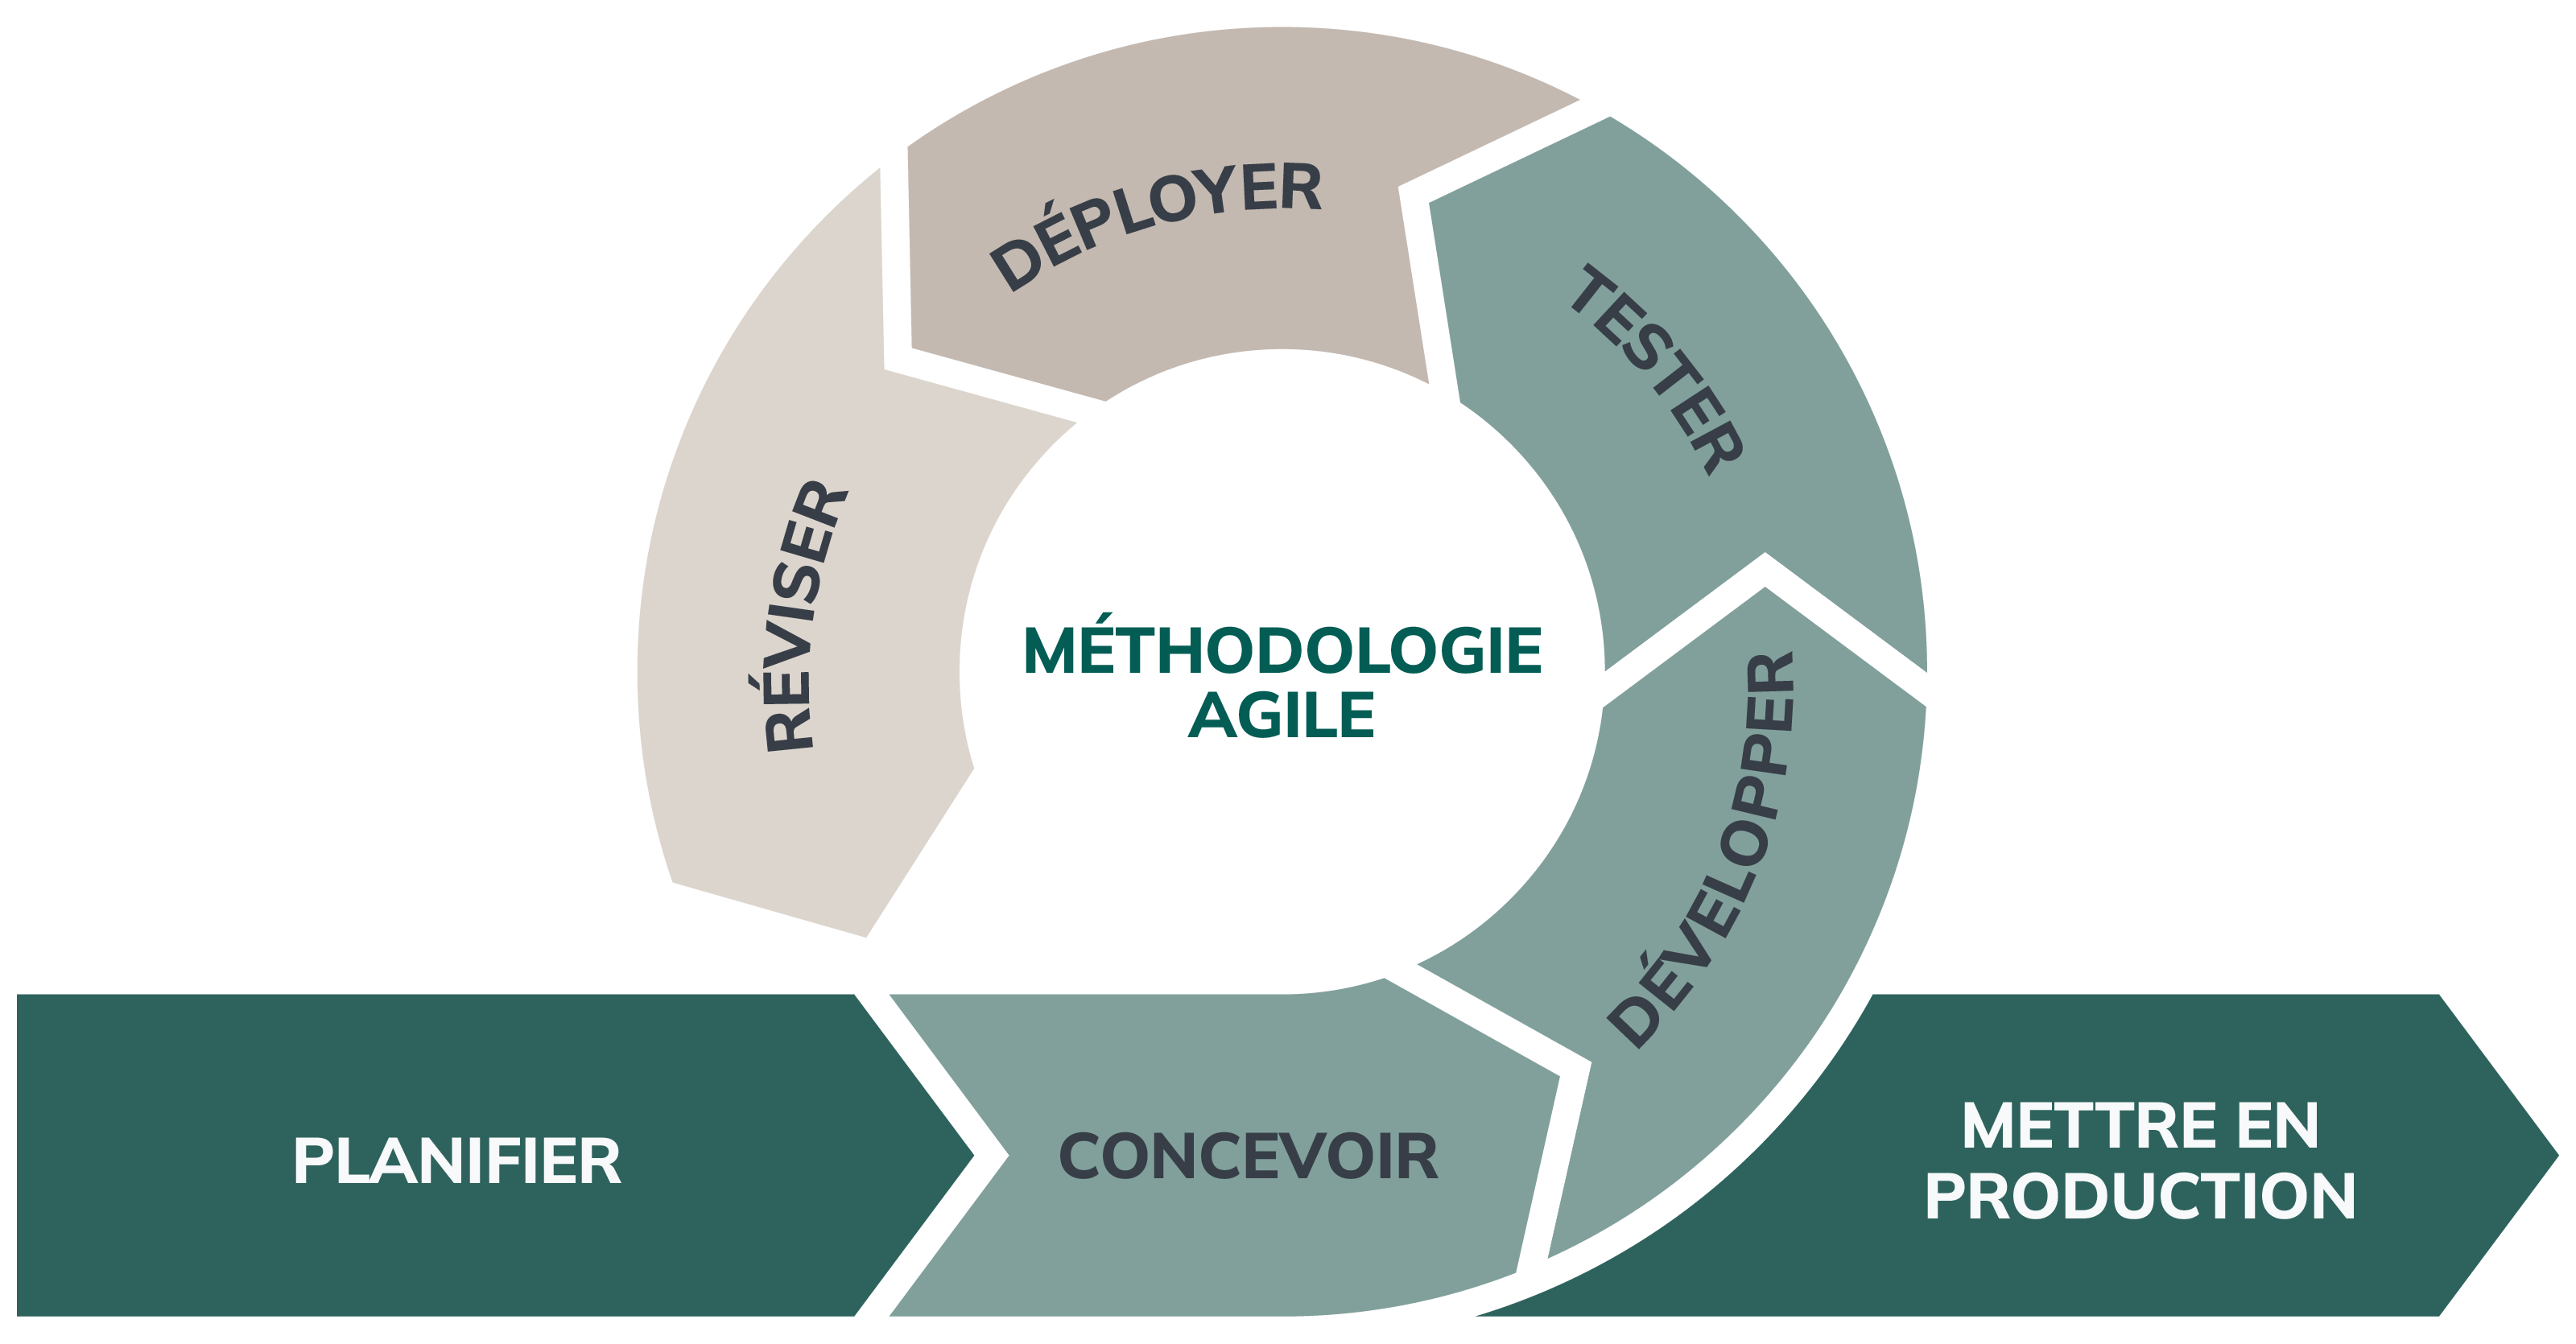
\includegraphics[scale=0.1]{project/images/Agile.png}
  \caption{Processus de méthodologie agile}
\end{figure}

\subsection{La méthodologie SCRUM}
Le framework \textbf{Scrum} repose sur une organisation du travail en cycles courts appelés \textbf{sprints}. Ces cycles, généralement d’une durée de deux semaines, permettent à l’équipe de produire à la fin de chaque itération un livrable exploitable appelé incrément. Chaque sprint possède une durée fixe, un objectif précis (Sprint Goal) ainsi qu’un périmètre défini à travers le Sprint \textbf{Backlog}.

Au début de chaque sprint, une réunion de planification (\textbf{Sprint Planning}) est organisée. Lors de cette réunion, l’équipe sélectionne, à partir du Backlog produit, les éléments qu’elle s’engage à réaliser durant le cycle en cours. Ces éléments constituent le Backlog de sprint. Le \textbf{Product Owner}, responsable de la vision du produit et de la gestion du Backlog produit, collabore avec l’équipe afin de clarifier les priorités et les attentes.

Durant le sprint, l’équipe de développement composée généralement de trois à huit membres travaille à transformer les besoins exprimés en fonctionnalités opérationnelles. Le \textbf{Scrum Master} veille au respect du cadre Scrum et facilite la collaboration au sein de l’équipe. Chaque jour, un \textbf{Daily Scrum} d’une durée de 15 minutes est organisé afin de synchroniser les membres, inspecter l’avancement des travaux et identifier d’éventuels obstacles.

À la fin du sprint, une \textbf{Sprint Review} est tenue pour présenter l’incrément réalisé et vérifier si l’objectif du sprint a été atteint. Cette réunion permet de recueillir les retours du client ou des parties prenantes, même si ces derniers ne font pas directement partie de l’équipe Scrum. Enfin, une rétrospective est organisée afin de prendre du recul, analyser le déroulement du sprint et identifier des axes d’amélioration pour les cycles suivants.

Ainsi, Scrum s’appuie sur les principes de transparence, d’inspection et d’adaptation, garantissant un processus itératif et évolutif centré sur l’amélioration continue et la création de valeur, comme l’illustre la figure 1.8.2 

\begin{figure}[H]
  \centering
    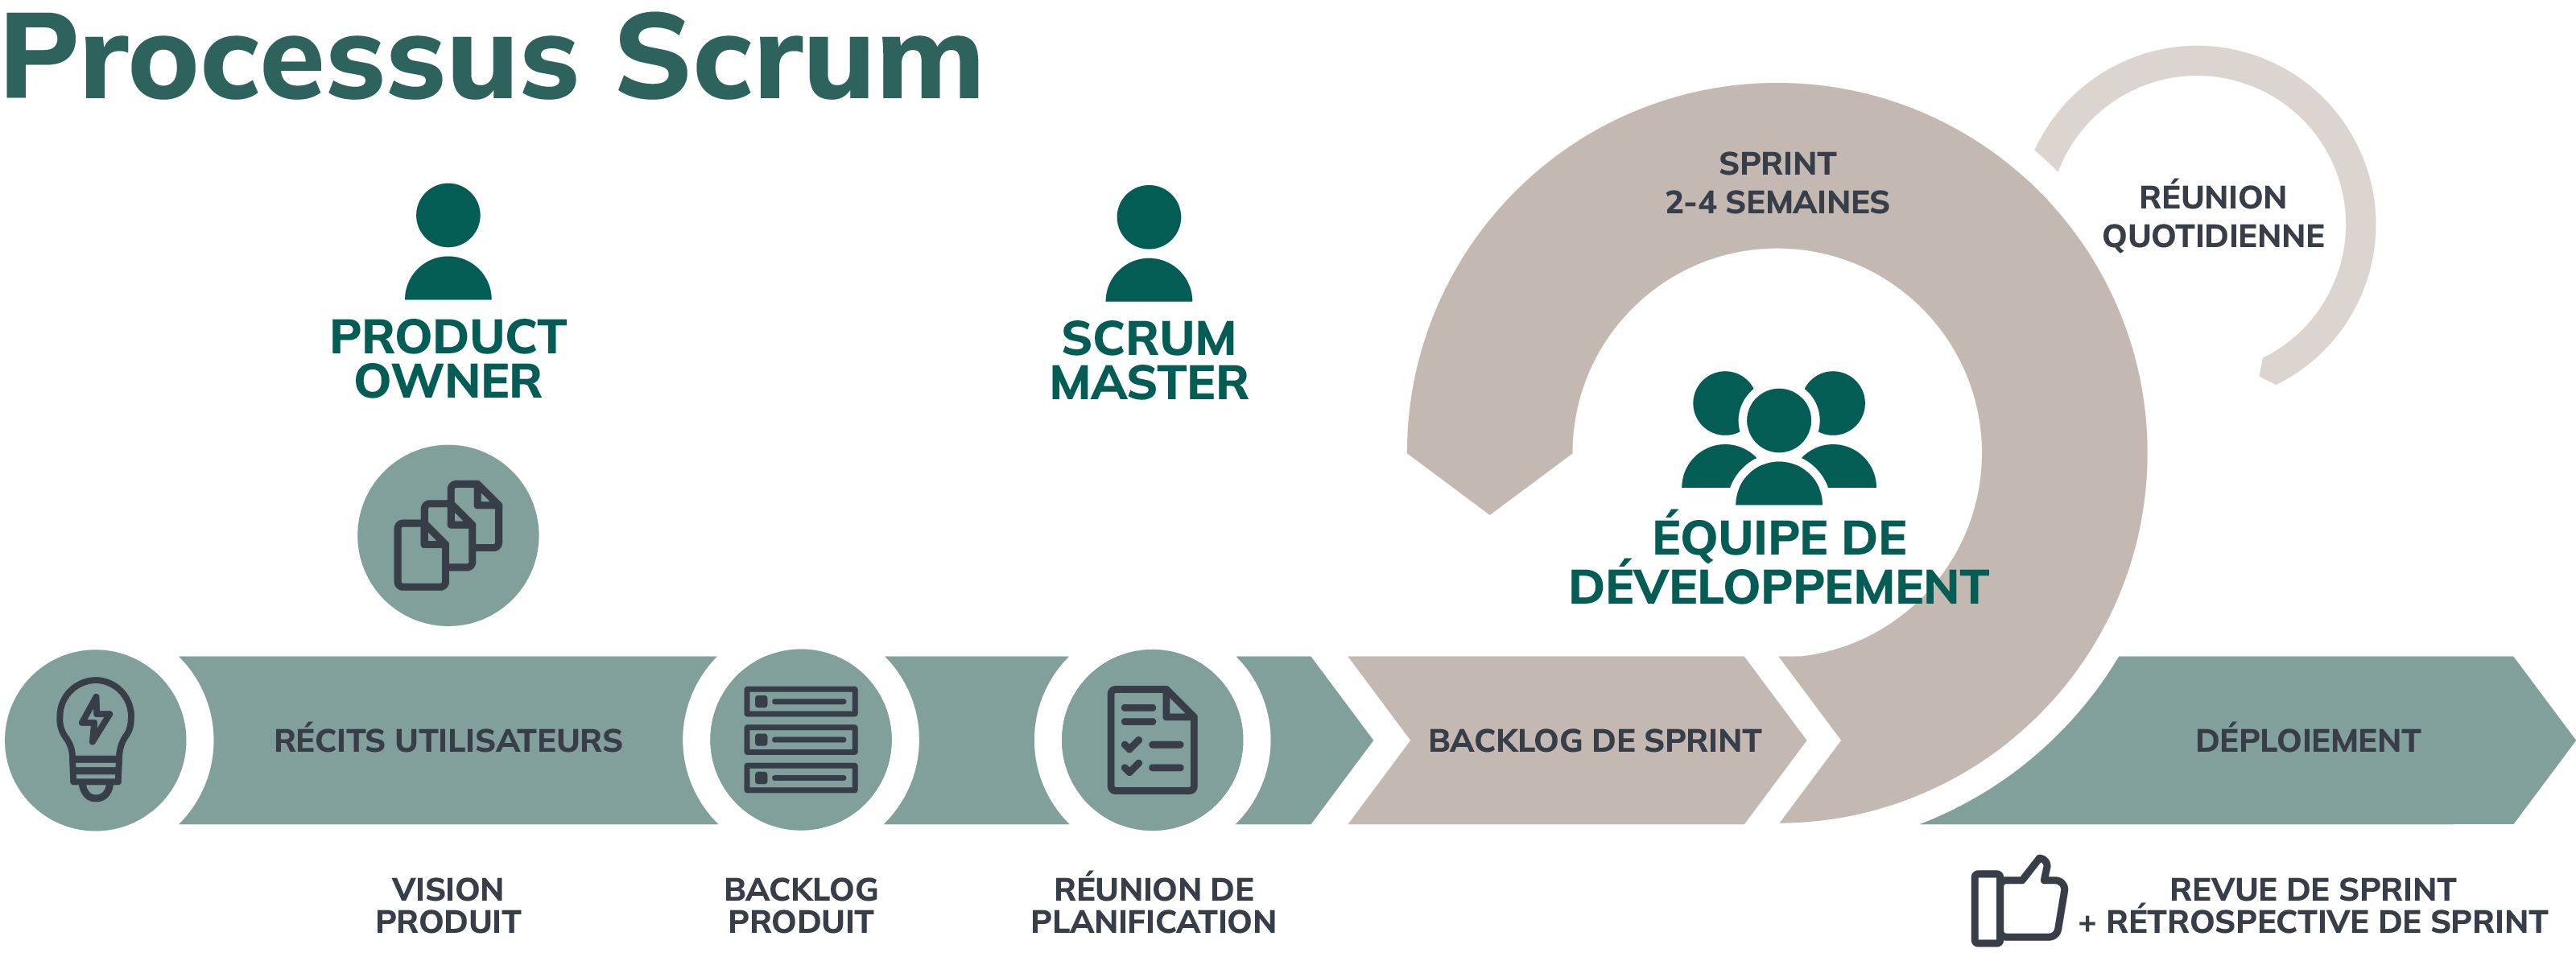
\includegraphics[scale=0.1]{project/images/scrum_agile.png}
  \caption{ Processus de la méthodologie SCRUM agile}
\end{figure}


\section{Conclusion}
Ce premier chapitre a permis de poser les bases de notre projet en présentant l'organisme d'accueil, son contexte et les défis auxquels il fait face. À travers l'étude de l'existant, sNous avons analysé les outils utilisés et mis en évidence leurs principales limites , ce qui nous a permis de proposer des solutions concrètes et adaptées. Pour mener ce travail à bien, nous avons opté pour la méthodologie Scrum Agile, qui nous offre la flexibilité et l'agilité nécessaires pour avancer efficacement tout en restant à l'écoute des besoins. Forts de ces bases solides, nous sommes maintenant prêts à passer à la conception et à la mise en œuvre de notre solution.




 







